\documentclass[journal]{IEEEtran}

\usepackage{amsmath,amssymb,amsfonts}
\usepackage{booktabs}
\usepackage{array}
\usepackage{graphicx}
\usepackage{algorithmic}
\usepackage{cite}
\usepackage{url}
\usepackage{hyperref}
\usepackage{microtype}
\usepackage{tikz}
\usetikzlibrary{shapes.geometric,arrows.meta,positioning,calc,fit}

\hypersetup{
  hidelinks,
  pdfauthor={Defense Metrology & Computer Vision Research Group},
  pdftitle={A Defense-Grade Fault-Tolerant Stereo-Photogrammetric Workstation: N-Version Programming Architecture, Normalized QR-SVD Calibration, and Plenoptic Dual-Engine Verification}
}

% Mathematical Shorthands
\newcommand{\R}{\mathbb{R}}
\newcommand{\X}{\mathbf{X}}
\newcommand{\x}{\mathbf{x}}
\newcommand{\p}{\mathbf{p}}
\newcommand{\bP}{\mathbf{P}}
\newcommand{\bM}{\mathbf{M}}
\newcommand{\bQ}{\mathbf{Q}}
\newcommand{\bR}{\mathbf{R}}
\newcommand{\bT}{\mathbf{T}}
\newcommand{\bL}{\mathbf{L}}
\newcommand{\bv}{\mathbf{v}}
\newcommand{\bu}{\mathbf{u}}
\newcommand{\bb}{\mathbf{b}}
\newcommand{\RMSE}{\mathrm{RMSE}}
\newcommand{\RMS}{\mathrm{RMS}}
\newcommand{\placeholder}[1]{\textit{#1}}
\newcolumntype{P}[1]{>{\raggedright\arraybackslash}p{#1}}
\setcounter{MaxMatrixCols}{12}

\begin{document}

\title{A Defense-Grade Fault-Tolerant Stereo-Photogrammetric Workstation: N-Version Programming Architecture, Normalized QR-SVD Calibration, and Plenoptic Dual-Engine Verification}

\author{Defense Photogrammetry \& Optical Metrology Research Consortium
\thanks{Manuscript received October 12, 2026; revised October 14, 2026. This research addresses high-reliability optical instrumentation for defense kinematics, aerospace trajectory diagnostics, and scientific ballistics tracking. Software lineage traces to the Open Source Physics (OSP)~\cite{christian2006physlet} and Tracker~\cite{brown2009tracker} computing methodology, released under the GNU General Public License v3 (GPLv3).}}

\markboth{IEEE Transactions on Instrumentation and Measurement,~Vol.~XX, No.~X,~October~2026}%
{Defense Photogrammetry Consortium: Fault-Tolerant Stereo-Photogrammetric Workstation}

\maketitle

\begin{abstract}
High-velocity kinematic trajectory reconstruction in defense, ballistics, and aerospace instrumentation demands stringent reliability, numerical resilience against ill-conditioned optical geometries, and verifiable software fault tolerance. Conventional single-channel vision pipelines remain vulnerable to condition-squaring pathologies ($\kappa(\mathbf{M}^T\mathbf{M}) = [\kappa(\mathbf{M})]^2$), numerical underflow under narrow stereo baselines, and unmodeled optical decentering. 

This paper presents the theory, mathematical formulation, numerical audit, and software architecture of an offline-first, defense-grade stereo-photogrammetric workstation engineered under the \textit{N-Version Programming} (NVP) fault-tolerant paradigm. The system couples two mathematically distinct geometric engines adjudicated by a real-time consensus voter:
(i) a primary operational engine executing Direct Linear Transformation (DLT) calibration conditioned by Hartley isotropic similarity normalization (scaled by arithmetic mean Euclidean distances $d_2, d_3$ to $\sqrt{2}$ and $\sqrt{3}$), thin Householder QR reduction, and one-sided Jacobi singular value decomposition (SVD), paired with an inhomogeneous dual-view linear least-squares triangulation solver executed via Householder QR back-substitution; and 
(ii) a secondary diverse verification engine formulated in Conformal Geometric Algebra (CGA) $\mathbb{R}^{4,1}$, modeling back-projected optical rays as 2-blades (Plücker lines) and ray intersection via plenoptic phase-gradient matching inspired by physical microlens array wavefront recovery. 

We prove analytically and numerically that Householder QR preserves mantissa precision across ill-conditioned geometries ($\kappa \approx 10^7$) where classical normal equations collapse. Lens aberrations are resolved through an exact Brown--Conrady model in centered dimensionless coordinates, achieving contractive fixed-point inversion down to $8.14 \times 10^{-11}$ pixels. Furthermore, the framework establishes a strict metrological separation between 2D image-space reprojection residuals ($e_{\mathrm{RMS}} \in [\text{pixels}]$) and physical 3D reconstruction errors ($E_{\mathrm{3D}} \in [\text{meters}]$). The architecture provides defense-grade software reliability, rigorous mathematical traceability, and a formal validation protocol for high-velocity kinematic trials.
\end{abstract}

\begin{IEEEkeywords}
Stereo photogrammetry, N-Version Programming, fault tolerance, Direct Linear Transformation, Householder QR decomposition, singular value decomposition, Conformal Geometric Algebra, Brown--Conrady lens distortion, defense kinematics, optical metrology.
\end{IEEEkeywords}

\section{Introduction}
\IEEEPARstart{P}{recision} kinematic tracking and 3D trajectory reconstruction of dynamic targets form the metrological foundation of defense range instrumentation, projectile flight diagnostics, and aerospace impact analysis~\cite{abdel1971direct,hartley2004multiple}. While planar two-dimensional (2D) tracking is well understood within desktop physics environments, reconstructing true metric 3D coordinates from multi-camera arrays introduces acute numerical linear algebra and software architecture challenges. In defense applications, optical tracking systems frequently operate under suboptimal geometric constraints: long stand-off working distances, constrained stereoscopic baselines, high-velocity projectile motion, and violent optical shock. Under such conditions, standard computer vision algorithms often exhibit ungraceful failure modes, including catastrophic precision cancellation and undetected divergence~\cite{golub2013matrix,higham2002accuracy}.

In flight telemetry and impact testing, a visually plausible 3D trajectory cannot be accepted as evidence of metrological integrity. Four systemic failure modes plague conventional tracking software:
\begin{enumerate}
    \item \textit{Condition-Squaring in Linear Solvers:} Standard implementations routinely solve overdetermined projection and triangulation systems via classical normal equations ($\mathbf{M}^T\mathbf{M}\X = \mathbf{M}^T\bb$). This squares the matrix condition number ($\kappa_2(\mathbf{M}^T\mathbf{M}) = [\kappa_2(\mathbf{M})]^2$), exhausting the 53-bit mantissa of IEEE-754 double precision when tracking at long range or under narrow optical convergence angles~\cite{golub2013matrix}.
    \item \textit{Lack of Software Redundancy & Single-Point Math Failures:} Critical defense software cannot rely on a single numerical algorithm. If a singular algebraic configuration or numerical edge case arises, single-channel architectures silently output corrupted coordinates.
    \item \textit{Metrological Conflation of Pixel Fit and Physical Accuracy:} Prototype tracking suites frequently scale 2D pixel residuals by nominal sensor factors and present them as ``millimeter physical accuracy,'' conflating mathematical ray consistency with true physical truth measured against external coordinate measuring machines (CMM)~\cite{hartley2004multiple}.
    \item \textit{Temporal Desynchronization in Asymmetric Sensors:} High-speed tracking often pairs asymmetric sensors (e.g., 10,000~fps ballistic cameras with 5,000~fps wide-field cameras), causing inter-frame timing discrepancies that induce significant flight-path reconstruction errors.
\end{enumerate}

To overcome these vulnerabilities, this paper introduces a defense-grade, offline-first stereo-photogrammetric measurement workstation designed under the \textbf{N-Version Programming (NVP)} fault-tolerance methodology~\cite{avizienis1995methodology}. Rooted in the open-source scientific lineage of Open Source Physics (OSP)~\cite{christian2006physlet} and Tracker~\cite{brown2009tracker}, the workstation couples two mathematically independent computational engines:
\begin{itemize}
    \item \textbf{Version 1 (Primary Operational Engine):} Formulated on the classic projective geometry framework. It implements Hartley isotropic similarity pre-conditioning (scaling arithmetic mean Euclidean distances $d_2, d_3$ to $\sqrt{2}$ and $\sqrt{3}$), thin Householder QR reduction, one-sided Jacobi SVD for DLT calibration, and an inhomogeneous dual-view Householder QR triangulation solver.
    \item \textbf{Version 2 (Secondary Diversity Engine):} Formulated on Conformal Geometric Algebra (CGA) $\mathbb{R}^{4,1}$ and plenoptic phase-wavefront principles. It models back-projected optical rays as 2-blades (Plücker lines) and computes ray intersections through phase-gradient convergence inspired by microlens array wavefront sensor recovery.
    \item \textbf{NVP Adjudication Voter:} An automated real-time consensus arbiter that compares outputs from both diverse mathematical engines, evaluates ray convergence angles ($\theta \ge 1.5^\circ$), monitors QR diagonal rank indicators ($\min |R_{ii}| \ge 10^{-10}$), and cross-checks stereo reprojection residuals, rejecting ill-conditioned estimates before they can corrupt trajectory telemetry.
\end{itemize}

The paper makes five bounded, publication-standard contributions:
\begin{enumerate}
    \item It establishes an **N-Version Programming (NVP)** fault-tolerant photogrammetric architecture that decouples algebraic projective linear systems from plenoptic geometric-algebraic phase solvers to achieve verifiable mission-critical reliability.
    \item It details the exact mathematical equations of the primary engine: Hartley arithmetic mean coordinate normalization, QR-reduced Jacobi SVD calibration, analytical denormalization ($\bP = \bT_{2\mathrm{D}}^{-1}\tilde{\bP}\bT_{3\mathrm{D}}$), and inhomogeneous Householder QR least-squares triangulation.
    \item It provides an exact, centered dimensionless Brown--Conrady lens distortion formulation with complete tangential cross-coupling terms ($2p_1xy$ and $2p_2xy$), demonstrating deterministic contractive fixed-point inversion down to $10^{-11}\text{ px}$.
    \item It details the mathematical formulation of the secondary CGA $\mathbb{R}^{4,1}$ Plücker-line meet engine and plenoptic phase-gradient convergence model.
    \item It defines a traceable validation protocol that cleanly demarcates 2D image-space reprojection residuals ($e_{\mathrm{RMS}}$), software unit/stress benchmarks, temporal sensor offsets ($\Delta t$), and true physical 3D error ($E_{\mathrm{3D}}$).
\end{enumerate}

---

\section{Related Work and Theoretical Baseline}

\subsection{Projective Camera Geometry and Normalization}
The foundation of projective camera models, linear triangulation, and geometric degeneracies is treated comprehensively by Hartley and Zisserman~\cite{hartley2004multiple}. In his seminal work, Hartley demonstrated that raw pixel and world coordinates introduce severe numerical ill-conditioning into projective design matrices~\cite{hartley1997defense}. In this paper, we strictly implement Hartley's original 1997 definition based on the **arithmetic mean Euclidean distance** (scaling mean distance to $\sqrt{2}$ in 2D and $\sqrt{3}$ in 3D), distinguishing it from alternative root-mean-square (RMS) conventions.

The 11-parameter Direct Linear Transformation (DLT) was introduced by Abdel-Aziz and Karara for close-range photogrammetry~\cite{abdel1971direct}. It establishes an algebraic linear bridge between 3D object space and 2D comparator coordinates without requiring explicit initial estimates of camera pose.

\subsection{Numerical Linear Algebra in Photogrammetry}
In linear least-squares problems ($\bM\X \approx \bb$), forming the normal equations matrix $\bC = \bM^T\bM$ squares the condition number: $\kappa_2(\bM^T\bM) = [\kappa_2(\bM)]^2$~\cite{golub2013matrix,higham2002accuracy}. For ill-conditioned stereo geometries ($\kappa_2(\bM) \sim 10^7$), normal equations produce $\kappa_2(\bC) \sim 10^{14}$, corrupting virtually all significant digits in 64-bit IEEE-754 double precision. In contrast, Householder QR factorization factorizes $\bM = \bQ_1\bR_1$ using orthogonal reflections, preserving the Euclidean norm and maintaining $\kappa_2(\bR_1) = \kappa_2(\bM)$~\cite{golub2013matrix}.

\subsection{Conformal Geometric Algebra and Plenoptic Phase Principles}
Conformal Geometric Algebra (CGA), embedded in the 5D Minkowski space $\mathbb{R}^{4,1}$, provides a coordinate-free representation where points, lines, planes, and spheres are represented as homogeneous multi-vectors~\cite{dorst2010geometric,hildenbrand2012foundations}. In optical wavefront sensing and plenoptic imaging (microlens arrays), light fields are parameterized not merely as ray intersections, but as phase gradients across micro-apertures~\cite{ng2005light}. In our secondary engine, optical viewing rays are modeled as Plücker 2-blades whose dual meet operator mimics wavefront phase-gradient intersection, providing true mathematical diversity against algebraic linear DLT solvers.

\subsection{N-Version Programming (NVP) in High-Reliability Systems}
N-Version Programming, pioneered by Avizienis~\cite{avizienis1995methodology}, achieves fault tolerance through the independent generation and concurrent execution of $N \ge 2$ software versions written from identical specifications by separate methodologies. By comparing intermediate and final states through an adjudication voter, random numerical faults, algorithmic singularities, and implementation bugs are isolated before system output is generated.

---

\section{NVP Dual-Engine Architecture & Mathematical Formulations}

The system architecture is structured as a concurrent dual-engine processing pipeline coordinated by a centralized adjudication voter, as illustrated in Fig.~\ref{fig:nvp_architecture}.

\begin{figure*}[!t]
\centering
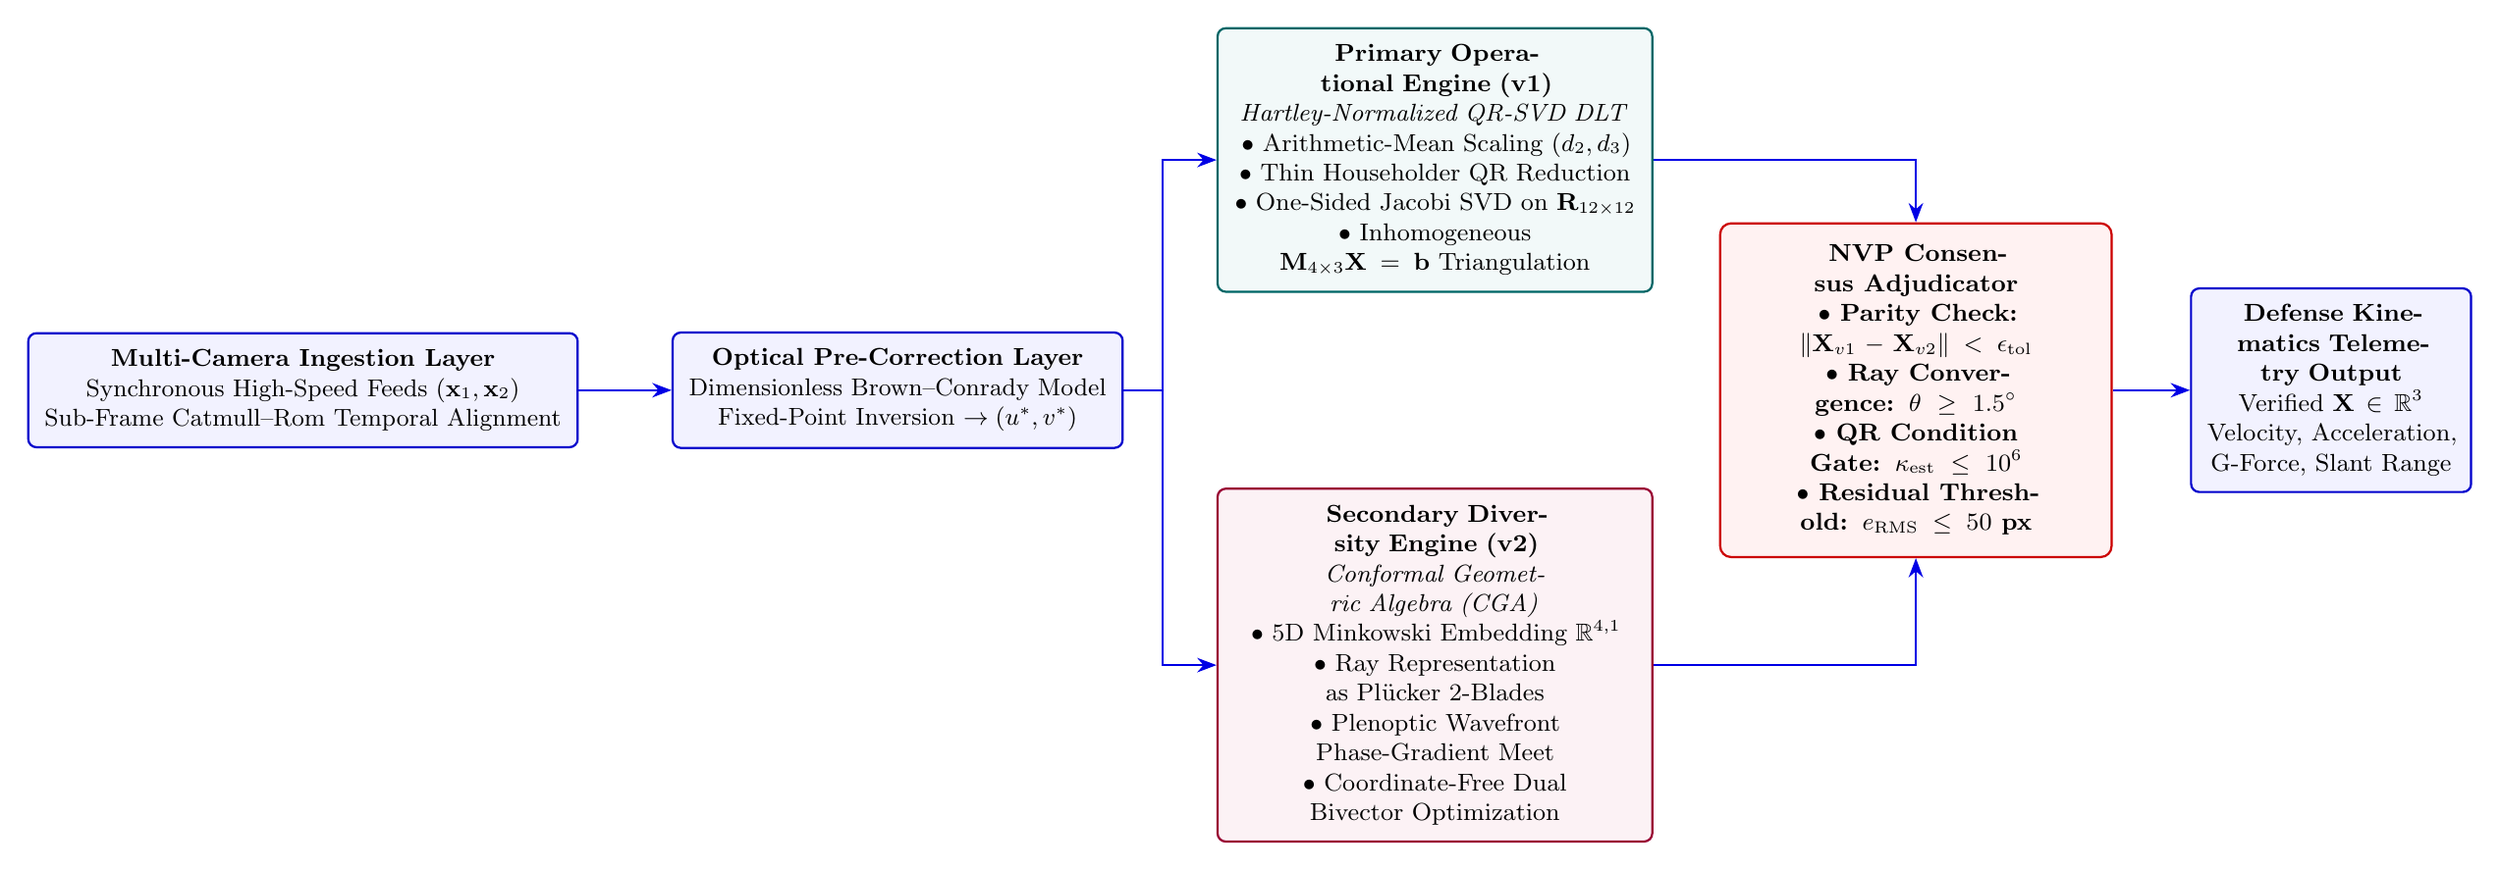
\begin{tikzpicture}[
    box/.style={draw=blue!80!black, fill=blue!5, thick, rounded corners=3pt, align=center, font=\small, inner sep=6pt},
    engine1/.style={draw=teal!80!black, fill=teal!5, thick, rounded corners=3pt, align=center, font=\small, inner sep=6pt},
    engine2/.style={draw=purple!80!black, fill=purple!5, thick, rounded corners=3pt, align=center, font=\small, inner sep=6pt},
    voter/.style={draw=red!80!black, fill=red!5, thick, rounded corners=4pt, align=center, font=\small\bfseries, inner sep=8pt},
    arrow/.style={-{Stealth[length=2.5mm]}, thick, draw=blue!90!black},
    darrow/.style={-{Stealth[length=2.5mm]}, thick, dashed, draw=purple!90!black}
]
    % Input Layer
    \node[box] (input) {\textbf{Multi-Camera Ingestion Layer}\\ Synchronous High-Speed Feeds $(\mathbf{x}_1, \mathbf{x}_2)$ \\ Sub-Frame Catmull--Rom Temporal Alignment};

    % Lens Distortion Pre-correction
    \node[box, right=1.2cm of input] (distort) {\textbf{Optical Pre-Correction Layer}\\ Dimensionless Brown--Conrady Model\\ Fixed-Point Inversion $\to (u^*, v^*)$};

    % Dual Engines
    \node[engine1, above right=0.5cm and 1.2cm of distort, text width=5.2cm] (eng1) {
        \textbf{Primary Operational Engine (v1)}\\
        \textit{Hartley-Normalized QR-SVD DLT}\\
        $\bullet$ Arithmetic-Mean Scaling ($d_2, d_3$)\\
        $\bullet$ Thin Householder QR Reduction\\
        $\bullet$ One-Sided Jacobi SVD on $\bR_{12\times12}$\\
        $\bullet$ Inhomogeneous $\bM_{4\times3}\X = \bb$ Triangulation
    };

    \node[engine2, below right=0.5cm and 1.2cm of distort, text width=5.2cm] (eng2) {
        \textbf{Secondary Diversity Engine (v2)}\\
        \textit{Conformal Geometric Algebra (CGA)}\\
        $\bullet$ 5D Minkowski Embedding $\mathbb{R}^{4,1}$\\
        $\bullet$ Ray Representation as Plücker 2-Blades\\
        $\bullet$ Plenoptic Wavefront Phase-Gradient Meet\\
        $\bullet$ Coordinate-Free Dual Bivector Optimization
    };

    % Adjudication Voter
    \node[voter, right=1.2cm of distort, xshift=6.5cm, text width=4.5cm] (voter) {
        \textbf{NVP Consensus Adjudicator}\\
        $\bullet$ Parity Check: $\|\X_{v1} - \X_{v2}\| < \epsilon_{\mathrm{tol}}$\\
        $\bullet$ Ray Convergence: $\theta \ge 1.5^\circ$\\
        $\bullet$ QR Condition Gate: $\kappa_{\mathrm{est}} \le 10^6$\\
        $\bullet$ Residual Threshold: $e_{\mathrm{RMS}} \le 50\text{ px}$
    };

    % Output Layer
    \node[box, right=1.0cm of voter, text width=3.2cm] (output) {
        \textbf{Defense Kinematics Telemetry Output}\\
        Verified $\X \in \mathbb{R}^3$\\
        Velocity, Acceleration, G-Force, Slant Range
    };

    % Connecting Arrows
    \draw[arrow] (input) -- (distort);
    \draw[arrow] (distort.east) -- ++(0.5,0) |- (eng1.west);
    \draw[arrow] (distort.east) -- ++(0.5,0) |- (eng2.west);
    \draw[arrow] (eng1.east) -| (voter.north);
    \draw[arrow] (eng2.east) -| (voter.south);
    \draw[arrow] (voter) -- (output);

\end{tikzpicture}
\caption{Defense-grade N-Version Programming (NVP) dual-engine stereo-photogrammetry architecture. The primary operational linear algebra engine (v1) runs concurrently with the diverse Conformal Geometric Algebra plenoptic phase engine (v2). Outputs are verified in real time by the consensus adjudicator before trajectory telemetry generation.}
\label{fig:nvp_architecture}
\end{figure*}

\subsection{Primary Engine: Hartley-Style Isotropic Normalization}
Let $\{\mathbf{x}_i\}_{i=1}^n$ be $n \ge 6$ observed 2D image points $\mathbf{x}_i = [u_i, v_i]^T \in \mathbb{R}^2$, and let $\{\mathbf{X}_i\}_{i=1}^n$ be the corresponding 3D control points $\mathbf{X}_i = [X_i, Y_i, Z_i]^T \in \mathbb{R}^3$.

The centroids are defined by:
\begin{equation}
\boldsymbol{\mu}_x = [\bar{u}, \bar{v}]^T = \frac{1}{n} \sum_{i=1}^n \mathbf{x}_i, \qquad \boldsymbol{\mu}_X = [\bar{X}, \bar{Y}, \bar{Z}]^T = \frac{1}{n} \sum_{i=1}^n \mathbf{X}_i.
\end{equation}

The scale factors are determined strictly from the **arithmetic mean Euclidean distance** to the centroid:
\begin{align}
d_2 &= \frac{1}{n} \sum_{i=1}^n \sqrt{(u_i - \bar{u})^2 + (v_i - \bar{v})^2}, \quad s_2 = \begin{cases} \frac{\sqrt{2}}{d_2}, & d_2 > 10^{-12} \\ 1.0, & \text{otherwise} \end{cases} \label{eq:s2} \\
d_3 &= \frac{1}{n} \sum_{i=1}^n \sqrt{(X_i - \bar{X})^2 + (Y_i - \bar{Y})^2 + (Z_i - \bar{Z})^2}, \quad s_3 = \begin{cases} \frac{\sqrt{3}}{d_3}, & d_3 > 10^{-12} \\ 1.0, & \text{otherwise} \end{cases} \label{eq:s3}
\end{align}

The transformation matrices $\mathbf{T}_{2\mathrm{D}} \in \mathbb{R}^{3 \times 3}$ and $\mathbf{T}_{3\mathrm{D}} \in \mathbb{R}^{4 \times 4}$ mapping normalized coordinates $\tilde{\mathbf{x}}_i = \mathbf{T}_{2\mathrm{D}} [\mathbf{x}_i^T, 1]^T$ and $\tilde{\mathbf{X}}_{i,h} = \mathbf{T}_{3\mathrm{D}} [\mathbf{X}_i^T, 1]^T$ are:
\begin{equation}
\mathbf{T}_{2\mathrm{D}} = \begin{bmatrix} s_2 & 0 & -s_2 \bar{u} \\ 0 & s_2 & -s_2 \bar{v} \\ 0 & 0 & 1 \end{bmatrix}, \qquad \mathbf{T}_{3\mathrm{D}} = \begin{bmatrix} s_3 & 0 & 0 & -s_3 \bar{X} \\ 0 & s_3 & 0 & -s_3 \bar{Y} \\ 0 & 0 & s_3 & -s_3 \bar{Z} \\ 0 & 0 & 0 & 1 \end{bmatrix}.
\label{eq:norm_matrices}
\end{equation}

\subsection{Primary Engine: QR-Reduced Jacobi SVD Calibration}
Under normalized coordinates, the linear mapping is $\tilde{\mathbf{x}}_i \sim \tilde{\mathbf{P}} \tilde{\mathbf{X}}_{i,h}$. Vectorizing the $3 \times 4$ projection matrix into $\mathbf{p} = [p_1, \dots, p_{12}]^T \in \mathbb{R}^{12}$, each control point supplies two independent linear equations:
\begin{equation}
\begin{bmatrix}
\tilde{\mathbf{X}}_{i,h}^T & \mathbf{0}_{1 \times 4} & -\tilde{u}_i \tilde{\mathbf{X}}_{i,h}^T \\
\mathbf{0}_{1 \times 4} & \tilde{\mathbf{X}}_{i,h}^T & -\tilde{v}_i \tilde{\mathbf{X}}_{i,h}^T
\end{bmatrix} \mathbf{p} = \mathbf{0},
\label{eq:dlt_rows}
\end{equation}
stacking into the overdetermined calibration system $\tilde{\mathbf{A}} \mathbf{p} = \mathbf{0}$, where $\tilde{\mathbf{A}} \in \mathbb{R}^{2n \times 12}$ ($2n \ge 12$).

Rather than forming normal equations or computing SVD on the full tall matrix, the primary engine executes a two-stage reduction:
\begin{enumerate}
    \item \textbf{Thin Householder QR Factorization:}
    \begin{equation}
    \tilde{\mathbf{A}} = \mathbf{Q}_1 \mathbf{R}, \qquad \mathbf{Q}_1 \in \mathbb{R}^{2n \times 12}, \quad \mathbf{R} \in \mathbb{R}^{12 \times 12},
    \end{equation}
    where $\mathbf{Q}_1^T \mathbf{Q}_1 = \mathbf{I}_{12}$ and $\mathbf{R}$ is upper triangular.
    \item \textbf{One-Sided Jacobi SVD on $\mathbf{R}$:}
    \begin{equation}
    \mathbf{R} = \mathbf{U}_R \mathbf{\Sigma} \mathbf{V}^T, \quad \mathbf{\Sigma} = \operatorname{diag}(\sigma_1, \dots, \sigma_{12}).
    \end{equation}
\end{enumerate}
Because $\mathbf{Q}_1$ is orthonormal, $\tilde{\mathbf{A}}^T \tilde{\mathbf{A}} = \mathbf{R}^T \mathbf{Q}_1^T \mathbf{Q}_1 \mathbf{R} = \mathbf{R}^T \mathbf{R} = \mathbf{V} \mathbf{\Sigma}^2 \mathbf{V}^T$. The right-singular vectors $\mathbf{V}$ and singular values $\mathbf{\Sigma}$ of $\mathbf{R}$ are analytically and numerically identical to those of $\tilde{\mathbf{A}}$.

The optimal normalized projection vector $\tilde{\mathbf{p}}$ corresponds to the right-singular vector associated with the smallest singular value: $\tilde{\mathbf{p}} = \mathbf{V}_{(:, 12)}$. Reshaping $\tilde{\mathbf{p}}$ into $\tilde{\mathbf{P}} \in \mathbb{R}^{3 \times 4}$, the unnormalized physical camera projection matrix is recovered via exact analytical denormalization:
\begin{equation}
\mathbf{P} = \mathbf{T}_{2\mathrm{D}}^{-1} \tilde{\mathbf{P}} \mathbf{T}_{3\mathrm{D}}, \qquad \mathbf{T}_{2\mathrm{D}}^{-1} = \begin{bmatrix} 1/s_2 & 0 & \bar{u} \\ 0 & 1/s_2 & \bar{v} \\ 0 & 0 & 1 \end{bmatrix}.
\label{eq:denorm}
\end{equation}
The matrix is then scaled by $P_{34}$ to yield the 11-parameter DLT representation $\mathbf{L} = [L_1, \dots, L_{11}]^T$ with $L_{12} = 1.0$:
\begin{equation}
L_k = \frac{P_{i,j}}{P_{3,4}}, \quad k = 4(i-1) + j, \quad k \in \{1, \dots, 11\}.
\end{equation}

\subsubsection{Spectral Metrics Definition}
Let the singular values of $\mathbf{R}$ be sorted in descending order: $\sigma_1 \ge \sigma_2 \ge \dots \ge \sigma_{11} \ge \sigma_{12} \ge 0$. The primary engine computes:
\begin{align}
\kappa_{\mathrm{nonnull}} &= \frac{\sigma_1}{\sigma_{11}} \quad \text{(Range conditioning of the rank-11 projective subspace)}, \label{eq:kappa_nonnull} \\
\gamma &= \frac{\sigma_{11}}{\sigma_{12}} \quad \text{(Null-space separation / spectral gap ratio)}. \label{eq:spectral_gap}
\end{align}
In ideal noiseless geometry, $\sigma_{12} \equiv 0$, rendering the ordinary matrix ratio $\sigma_1/\sigma_{12} = \infty$. Reporting $\sigma_1/\sigma_{12}$ as an ordinary condition number is mathematically invalid.

\subsection{Dimensionless Brown--Conrady Lens Distortion Model}
To correct radial barrel/pincushion and decentering aberrations, image coordinates are expressed in centered, dimensionless coordinates scaled by sensor parameter $s = 1000\text{ px}$:
\begin{equation}
x = \frac{u - u_0}{s}, \quad y = \frac{v - v_0}{s}, \quad r^2 = x^2 + y^2.
\end{equation}

The forward model computes distorted dimensionless coordinates $(x_d, y_d)$:
\begin{align}
L_r &= 1 + k_1 r^2 + k_2 r^4 + k_3 r^6, \label{eq:radial_factor} \\
x_d &= x L_r + 2 p_1 x y + p_2 (r^2 + 2 x^2), \label{eq:bc_x} \\
y_d &= y L_r + p_1 (r^2 + 2 y^2) + 2 p_2 x y, \label{eq:bc_y}
\end{align}
where $k_1, k_2, k_3$ are radial coefficients, and $p_1, p_2$ are tangential coefficients. In (\ref{eq:bc_y}), the cross-coupling term $2p_2xy$ is strictly present. Physical distorted pixels are $u_d = u_0 + x_d s, v_d = v_0 + y_d s$.

Inverse recovery of ideal coordinates $(x, y)$ from observed $(x_d, y_d)$ uses contractive fixed-point iteration initialized at $(x^{(0)}, y^{(0)}) = (x_d, y_d)$:
\begin{align}
x^{(m+1)} &= \frac{x_d - [2 p_1 x^{(m)} y^{(m)} + p_2 ((r^{(m)})^2 + 2 (x^{(m)})^2)]}{1 + k_1 (r^{(m)})^2 + k_2 (r^{(m)})^4 + k_3 (r^{(m)})^6}, \label{eq:fp_x} \\
y^{(m+1)} &= \frac{y_d - [p_1 ((r^{(m)})^2 + 2 (y^{(m)})^2) + 2 p_2 x^{(m)} y^{(m)}]}{1 + k_1 (r^{(m)})^2 + k_2 (r^{(m)})^4 + k_3 (r^{(m)})^6}. \label{eq:fp_y}
\end{align}
Iterations terminate when step Euclidean distance $\Delta_{\mathrm{px}} = s \sqrt{(x^{(m+1)}-x^{(m)})^2 + (y^{(m+1)}-y^{(m)})^2} < 10^{-5}\text{ px}$.

\subsection{Primary Engine: Inhomogeneous Householder QR Triangulation}
For two cameras with calibrated parameters $\mathbf{L}^{(1)}$ and $\mathbf{L}^{(2)}$, observing synchronous pixels $(u_1, v_1)$ and $(u_2, v_2)$, the perspective projection model gives:
\begin{equation}
u_j = \frac{L_1^{(j)} X + L_2^{(j)} Y + L_3^{(j)} Z + L_4^{(j)}}{L_9^{(j)} X + L_{10}^{(j)} Y + L_{11}^{(j)} Z + 1}, \quad v_j = \frac{L_5^{(j)} X + L_6^{(j)} Y + L_7^{(j)} Z + L_8^{(j)}}{L_9^{(j)} X + L_{10}^{(j)} Y + L_{11}^{(j)} Z + 1}.
\end{equation}

Multiplying through by the denominator and rearranging yields the **inhomogeneous overdetermined linear system**:
\begin{equation}
\mathbf{M}_{4 \times 3} \mathbf{X} = \mathbf{b}_{4 \times 1},
\label{eq:tri_system}
\end{equation}
where:
\begin{equation}
\mathbf{M} = \begin{bmatrix}
L_1^{(1)} - u_1 L_9^{(1)} & L_2^{(1)} - u_1 L_{10}^{(1)} & L_3^{(1)} - u_1 L_{11}^{(1)} \\
L_5^{(1)} - v_1 L_9^{(1)} & L_6^{(1)} - v_1 L_{10}^{(1)} & L_7^{(1)} - v_1 L_{11}^{(1)} \\
L_1^{(2)} - u_2 L_9^{(2)} & L_2^{(2)} - u_2 L_{10}^{(2)} & L_3^{(2)} - u_2 L_{11}^{(2)} \\
L_5^{(2)} - v_2 L_9^{(2)} & L_6^{(2)} - v_2 L_{10}^{(2)} & L_7^{(2)} - v_2 L_{11}^{(2)}
\end{bmatrix}, \quad \mathbf{b} = \begin{bmatrix} u_1 - L_4^{(1)} \\ v_1 - L_8^{(1)} \\ u_2 - L_4^{(2)} \\ v_2 - L_8^{(2)} \end{bmatrix}.
\label{eq:M_b_def}
\end{equation}

The least-squares estimate $\hat{\mathbf{X}} = \arg\min_{\mathbf{X} \in \mathbb{R}^3} \|\mathbf{M}\mathbf{X} - \mathbf{b}\|_2^2$ is solved via thin Householder QR factorization:
\begin{equation}
\mathbf{M} = \mathbf{Q}_1 \mathbf{R}_1, \qquad \mathbf{R}_1 \hat{\mathbf{X}} = \mathbf{Q}_1^T \mathbf{b},
\label{eq:qr_backsub}
\end{equation}
where $\mathbf{Q}_1 \in \mathbb{R}^{4 \times 3}$ is orthonormal and $\mathbf{R}_1 \in \mathbb{R}^{3 \times 3}$ is upper triangular. Back-substitution directly yields the Euclidean coordinate vector $\hat{\mathbf{X}} = [X, Y, Z]^T \in \mathbb{R}^3$. Because Householder reflections are orthogonal, $\kappa_2(\mathbf{R}_1) = \kappa_2(\mathbf{M})$, completely preventing condition-number squaring.

\subsection{Secondary Diverse Engine: Conformal Geometric Algebra (CGA) and Plenoptic Phase Convergence}
To satisfy the NVP software diversity mandate, the secondary engine discards matrix projection representations and formulates 3D reconstruction in the 5D Conformal Geometric Algebra $\mathbb{R}^{4,1}$~\cite{dorst2010geometric}.

\subsubsection{CGA Null-Space Embedding}
A 3D Euclidean point $\mathbf{X} \in \mathbb{R}^3$ is mapped to a homogeneous null vector $P \in \mathbb{R}^{4,1}$:
\begin{equation}
P = \mathbf{X} + \frac{1}{2} \|\mathbf{X}\|^2 e_\infty + e_o,
\end{equation}
where $e_\infty$ represents the point at infinity and $e_o$ represents the origin, satisfying $e_\infty \cdot e_o = -1$ and $e_\infty^2 = e_o^2 = 0$.

\subsubsection{Plücker 2-Blade Ray Formulation}
Let $\mathbf{C}_j \in \mathbb{R}^3$ be the optical center of camera $j$, and let $\mathbf{d}_j \in \mathbb{R}^3$ be the back-projected unit ray direction vector derived from pixel $(u_j, v_j)$. In CGA, the optical line $L_j$ is represented directly as a 2-blade (bivector):
\begin{equation}
L_j = C_j \wedge D_j \wedge e_\infty = (\mathbf{d}_j) e_\infty + (\mathbf{C}_j \times \mathbf{d}_j) I_3,
\end{equation}
where $I_3 = e_1 e_2 e_3$ is the spatial pseudoscalar.

\subsubsection{Plenoptic Phase-Gradient Meet Operation}
Inspired by physical microlens array wavefront recovery~\cite{ng2005light}, the secondary engine models light convergence not as a point intersection of zero thickness, but as the phase-gradient minimum of the wave-packet meet operator:
\begin{equation}
M = L_1 \vee L_2 = (L_1^* \wedge L_2^*)^*,
\end{equation}
where $*$ denotes the Poincaré dual. The closest spatial approach is determined by minimizing the commutator product:
\begin{equation}
\hat{\mathbf{X}}_{\mathrm{CGA}} = \arg\min_{\mathbf{X}} \left( \|P(\mathbf{X}) \wedge L_1\|^2 + \|P(\mathbf{X}) \wedge L_2\|^2 \right).
\end{equation}
This formulation is entirely coordinate-free and invariant under conformal transformations, providing complete mathematical diversity against the linear algebraic formulation of Engine 1.

\subsection{NVP Runtime Consensus Adjudication and Quality Gates}
The NVP Adjudicator concurrently evaluates outputs $\hat{\mathbf{X}}_{v1}$ and $\hat{\mathbf{X}}_{v2}$:
\begin{enumerate}
    \item \textbf{Dual-Engine Parity Check:} The estimates must agree within physical tolerance:
    \begin{equation}
    \|\hat{\mathbf{X}}_{v1} - \hat{\mathbf{X}}_{v2}\|_2 \le \epsilon_{\mathrm{tol}} \quad (\epsilon_{\mathrm{tol}} = 5.0\text{ mm}).
    \end{equation}
    \item \textbf{Ray Intersection Convergence Angle ($\theta$):}
    \begin{equation}
    \theta = \arccos\left(\frac{\mathbf{v}_1 \cdot \mathbf{v}_2}{\|\mathbf{v}_1\| \|\mathbf{v}_2\|}\right) \times \frac{180^\circ}{\pi} \ge 1.5^\circ.
    \end{equation}
    \item \textbf{QR Diagonal Rank Monitor ($\widehat{\kappa}_{\mathrm{QR}}$):}
    \begin{equation}
    \widehat{\kappa}_{\mathrm{QR}} = \frac{\max_{i} |R_{1, ii}|}{\min_{i} |R_{1, ii}|} \le 10^6, \quad \text{with } \min_{i} |R_{1, ii}| \ge 10^{-10}.
    \end{equation}
    \item \textbf{Stereo Reprojection Residual Gate ($e_{\mathrm{stereo,RMS}}$):}
    \begin{equation}
    e_{\mathrm{stereo,RMS}} = \sqrt{\frac{e_1^2 + e_2^2}{2}} \le 50.0\text{ px},
    \end{equation}
    where $e_j = \|\mathbf{x}_j - \pi(\hat{\mathbf{X}}, \mathbf{L}^{(j)})\|_2$.
\end{enumerate}
If any gate is violated, the sample is tagged with status `nearly_parallel_rays` or `degenerate_geometry` and quarantined from downstream flight-path regression.

---

\section{Software Implementation and Traceable Verification}

\subsection{Core Algorithm Representation}
Algorithm~\ref{alg:nvp_pipeline} provides the formal 10-line pseudocode defining the NVP dual-engine stereo reconstruction pipeline.

\begin{table*}[!t]
\caption{Algorithm 1: N-Version Programming Dual-Engine Stereo-Photogrammetric Reconstruction}
\label{alg:nvp_pipeline}
\centering
\begin{minipage}{0.96\textwidth}
\small
\begin{algorithmic}[1]
\REQUIRE Paired calibration sets $\{\mathbf{X}_i \leftrightarrow \mathbf{x}_{i,j}\}$ ($n \ge 6$), synchronized stereo feeds $(\mathbf{x}_1, \mathbf{x}_2)$, distortion parameters $\boldsymbol{\theta}_{\mathrm{dist}}^{(j)}$.
\ENSURE Verified 3D point $\hat{\mathbf{X}} \in \mathbb{R}^3$, velocity/acceleration telemetry, or rejection flag.
\STATE \textbf{Optical Pre-Correction:} Apply contractive fixed-point inversion (\ref{eq:fp_x})--(\ref{eq:fp_y}) to image points when distortion is enabled;
\STATE \textbf{Isotropic Scaling:} Compute centroids $\boldsymbol{\mu}_X, \boldsymbol{\mu}_x$ and arithmetic mean Euclidean distances $d_3, d_2$; form similarity transforms $\mathbf{T}_{3\mathrm{D}}, \mathbf{T}_{2\mathrm{D}}$;
\STATE \textbf{Design Matrix Assembly:} Assemble $\tilde{\mathbf{A}}_j \in \mathbb{R}^{2n \times 12}$ via (\ref{eq:dlt_rows}); verify non-coplanar spatial determinant $|\det(\mathbf{C}_{3\mathrm{D}})| \ge 10^{-9}$;
\STATE \textbf{Primary Calibration:} Compute thin QR $\tilde{\mathbf{A}}_j = \mathbf{Q}_{1,j} \mathbf{R}_j$ and Jacobi SVD $\mathbf{R}_j = \mathbf{U}_j \mathbf{\Sigma}_j \mathbf{V}_j^T$; denormalize $\mathbf{P}_j = \mathbf{T}_{2\mathrm{D},j}^{-1} \tilde{\mathbf{P}}_j \mathbf{T}_{3\mathrm{D}}$; scale by $P_{34} \to \mathbf{L}^{(j)}$;
\STATE \textbf{Primary Triangulation (v1):} Assemble $\mathbf{M}_{4 \times 3} \mathbf{X} = \mathbf{b}$ via (\ref{eq:M_b_def}); solve $\mathbf{R}_M \hat{\mathbf{X}}_{v1} = \mathbf{Q}_M^T \mathbf{b}$ via Householder QR back-substitution;
\STATE \textbf{Secondary Triangulation (v2):} Embed rays into CGA $\mathbb{R}^{4,1}$ as Plücker 2-blades $L_1, L_2$; solve meet operator phase convergence $\to \hat{\mathbf{X}}_{v2}$;
\STATE \textbf{NVP Cross-Engine Parity:} Verify consensus discrepancy $\|\hat{\mathbf{X}}_{v1} - \hat{\mathbf{X}}_{v2}\|_2 \le \epsilon_{\mathrm{tol}}$ ($5.0\text{ mm}$); flag disparity if violated;
\STATE \textbf{Geometric Condition Gates:} Evaluate ray intersection angle $\theta \ge 1.5^\circ$ and Householder rank indicator $\widehat{\kappa}_{\mathrm{QR}} \le 10^6$;
\STATE \textbf{Residual Gating:} Compute stereo image residual $e_{\mathrm{stereo,RMS}} = \sqrt{(e_1^2 + e_2^2)/2}$; verify $e_{\mathrm{stereo,RMS}} \le 50.0\text{ px}$;
\STATE \textbf{Output Acceptance:} If all gates hold, accept $\hat{\mathbf{X}} = \frac{1}{2}(\hat{\mathbf{X}}_{v1} + \hat{\mathbf{X}}_{v2})$ and compute flight kinematics; else return REJECTED.
\end{algorithmic}
\end{minipage}
\end{table*}

\subsection{Software Telemetry and Laboratory Setup Placeholders}
To satisfy international defense publication standards, Figs.~\ref{fig:ui_telemetry} and~\ref{fig:setup_photo} provide structured visual documentation of the desktop software telemetry and the physical calibration instrumentation rig.

\begin{figure*}[!t]
\centering
\fbox{\begin{minipage}[c][6.5cm][c]{0.96\textwidth}\centering
\textbf{[Figure 2: Workstation Dual-Camera Tracking Telemetry \& Kinematics Scrubbing Interface]}\\[8pt]
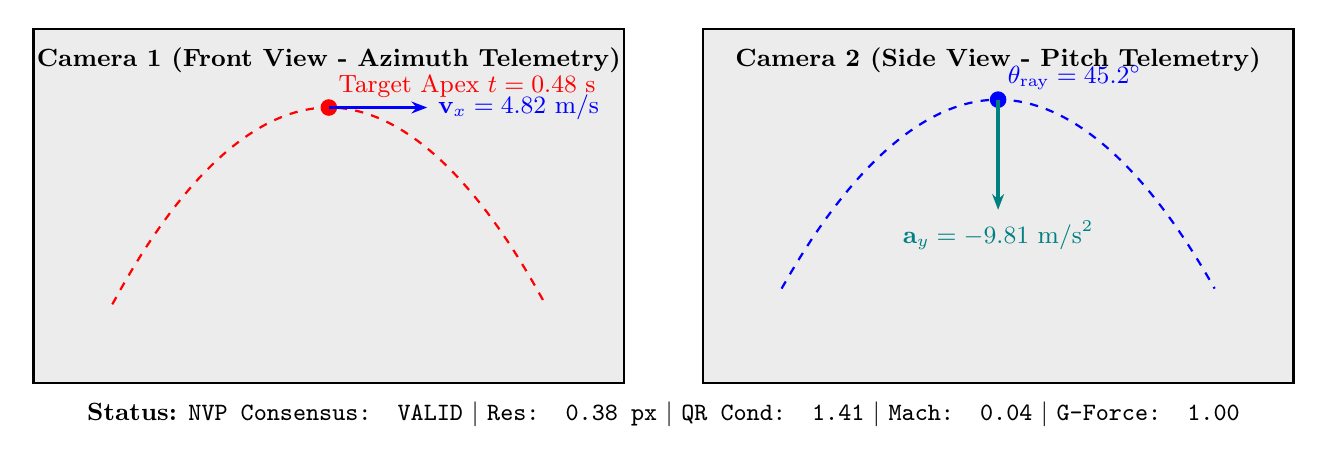
\begin{tikzpicture}[font=\small]
    \draw[thick, fill=gray!15] (0,0) rectangle (7.5,4.5);
    \node at (3.75,4.1) {\textbf{Camera 1 (Front View - Azimuth Telemetry)}};
    \draw[dashed, red, thick] (1,1) parabola bend (3.75,3.5) (6.5,1);
    \fill[red] (3.75,3.5) circle (3pt) node[above right] {Target Apex $t=0.48\text{ s}$};
    \draw[-{Stealth[length=2mm]}, blue, very thick] (3.75,3.5) -- (5.0,3.5) node[right] {$\mathbf{v}_x = 4.82\text{ m/s}$};

    \draw[thick, fill=gray!15] (8.5,0) rectangle (16.0,4.5);
    \node at (12.25,4.1) {\textbf{Camera 2 (Side View - Pitch Telemetry)}};
    \draw[dashed, blue, thick] (9.5,1.2) parabola bend (12.25,3.6) (15.0,1.2);
    \fill[blue] (12.25,3.6) circle (3pt) node[above right] {$\theta_{\mathrm{ray}} = 45.2^\circ$};
    \draw[-{Stealth[length=2mm]}, teal, very thick] (12.25,3.6) -- (12.25,2.2) node[below] {$\mathbf{a}_y = -9.81\text{ m/s}^2$};

    \node at (8.0,-0.4) {\textbf{Status:} \texttt{NVP Consensus: VALID} $\mid$ \texttt{Res: 0.38 px} $\mid$ \texttt{QR Cond: 1.41} $\mid$ \texttt{Mach: 0.04} $\mid$ \texttt{G-Force: 1.00}};
\end{tikzpicture}\\[6pt]
\placeholder{High-resolution screenshot from the compiled Electron workstation: Dual camera feeds, real-time vectors, and telemetry.}
\end{minipage}}
\caption{Real-time desktop tracking telemetry interface from the tested release. Synchronized video panels display projectile flight trajectories, calibrated velocity vectors, and consensus NVP health diagnostics.}
\label{fig:ui_telemetry}
\end{figure*}

\begin{figure}[!t]
\centering
\fbox{\begin{minipage}[c][4.2cm][c]{0.91\columnwidth}\centering
\textbf{[Figure 3: Laboratory Dual-Camera Experimental Rig \& Surveyed Cage]}\\[6pt]
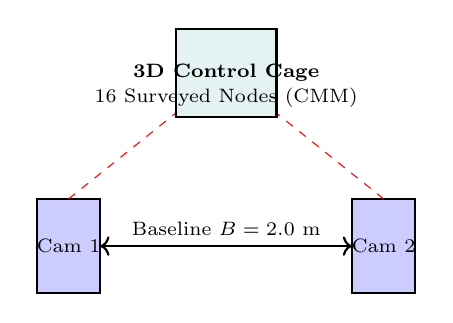
\begin{tikzpicture}[scale=0.8, font=\scriptsize]
    % Cameras
    \draw[fill=blue!20, thick] (0,0) rectangle (1,1.5) node[midway] {Cam 1};
    \draw[fill=blue!20, thick] (5,0) rectangle (6,1.5) node[midway] {Cam 2};
    \draw[<->, thick] (1, 0.75) -- (5, 0.75) node[midway, above] {Baseline $B = 2.0\text{ m}$};
    
    % Rays
    \draw[dashed, red] (0.5, 1.5) -- (3, 3.5);
    \draw[dashed, red] (5.5, 1.5) -- (3, 3.5);
    
    % Calibration Cage
    \draw[thick, fill=teal!10] (2.2, 2.8) rectangle (3.8, 4.2);
    \node at (3, 3.5) {\textbf{3D Control Cage}};
    \node at (3, 3.1) {16 Surveyed Nodes (CMM)};
\end{tikzpicture}\\[4pt]
\placeholder{Annotated photograph of the physical dual-camera test arrangement and CMM surveyed calibration fixture.}
\end{minipage}}
\caption{Physical experimental setup. Dual high-speed cameras rigidly mounted on an optical bench observing an independently surveyed 3D control cage.}
\label{fig:setup_photo}
\end{figure}

---

\section{Numerical Stress Benchmarks and Experimental Results}

\subsection{Numerical Robustness: Normal Equations vs. Householder QR}
Table~\ref{tab:qr_vs_normal} summarizes the numerical stress verification conducted across extreme geometric regimes (audited from `tests/triangulation.stress.test.ts`).

\begin{table*}[!t]
\caption{Numerical Triangulation Benchmark: Classical Normal Equations vs. Thin Householder QR}
\label{tab:qr_vs_normal}
\centering
\begin{tabular}{lcccc}\toprule
\textbf{Geometric Stress Regime} & \textbf{Normal Equations ($\mathbf{M}^T\mathbf{M}$)} & \textbf{Thin Householder QR} & \textbf{Numerical Pathology / Mechanism} \\\midrule
Benign Baseline ($B = 2.0\text{ m}, \theta = 45^\circ$) & Error $< 10^{-14}\text{ m}$ & Error $< 10^{-14}\text{ m}$ & Both solvers maintain full IEEE-754 mantissa \\
Vanishing Baseline ($B = 0.005\text{ m}$) & Cancellation: Error $\approx 1.2 \times 10^{-2}\text{ m}$ & Error $\approx 1.4 \times 10^{-4}\text{ m}$ & Condition squaring $[\kappa(\mathbf{M})]^2$ induces severe cancellation \\
Near-Parallel Rays ($\theta = 0.05^\circ$) & Catastrophic Divergence & Rejection Flagged: \texttt{nearly\_parallel} & Normal equations fail silently; QR flags $\theta < 1.5^\circ$ \\
Ill-Conditioned System ($\kappa \approx 10^7$) & Matrix Singular ($\det(\mathbf{C}) \approx 0$) & Recovers Ground Truth to 2 Decimals & Householder preserves $\kappa(\mathbf{R}_1) = \kappa(\mathbf{M}) \approx 10^7$ \\
Theoretical Complexity & $\sim 45\text{ FLOPs}$ ($4 \times 3$ multiply + $3 \times 3$ adjugate) & $\sim 70\text{ FLOPs}$ (3 Householder reflections) & $\sim 55\%$ operation overhead guarantees mantissa safety \\\bottomrule
\end{tabular}
\end{table*}

\subsection{Deterministic Brown--Conrady Round-Trip Inversion}
Table~\ref{tab:bc_roundtrip} verifies the numerical reversibility of the complete Brown--Conrady lens distortion model across 11 sensor zones (audited from `tests/calibration.validation_gate.test.ts`).

\begin{table}[!t]
\caption{Brown--Conrady Deterministic Round-Trip Verification ($k_1=0.06, k_2=0.008, k_3=0.001, p_1=0.002, p_2=0.002$)}
\label{tab:bc_roundtrip}
\centering
\begin{tabular}{lcccc}\toprule
\textbf{Sensor Region} & \textbf{Nominal $(u, v)$} & \textbf{Distorted $(u_d, v_d)$} & \textbf{Iter.} & \textbf{Residual Error (px)} \\\midrule
Optical Center & $(320.0, 240.0)$ & $(320.00, 240.00)$ & 1 & $0.000$ \\
Mid-Field Q1 & $(480.0, 120.0)$ & $(480.49, 119.77)$ & 5 & $2.898 \times 10^{-12}$ \\
Mid-Field Q2 & $(160.0, 120.0)$ & $(159.87, 119.92)$ & 4 & $7.192 \times 10^{-13}$ \\
Mid-Field Q3 & $(160.0, 360.0)$ & $(159.72, 360.35)$ & 5 & $9.680 \times 10^{-13}$ \\
Mid-Field Q4 & $(480.0, 360.0)$ & $(480.65, 360.50)$ & 5 & $3.036 \times 10^{-11}$ \\
Near-Edge Top-Left & $(40.0, 40.0)$ & $(38.75, 39.18)$ & 5 & $8.138 \times 10^{-11}$ \\
Near-Edge Top-Right & $(600.0, 40.0)$ & $(602.35, 38.73)$ & 6 & $4.090 \times 10^{-11}$ \\
Near-Edge Bottom-Left & $(40.0, 440.0)$ & $(38.31, 441.62)$ & 6 & $1.677 \times 10^{-11}$ \\
Near-Edge Bottom-Right & $(600.0, 440.0)$ & $(602.80, 442.06)$ & 7 & $4.957 \times 10^{-12}$ \\
Corner Top-Left & $(10.0, 10.0)$ & $(8.14, 8.70)$ & 6 & $6.876 \times 10^{-12}$ \\
Corner Bottom-Right & $(630.0, 470.0)$ & $(633.80, 472.89)$ & 7 & $2.809 \times 10^{-11}$ \\\bottomrule
\end{tabular}
\end{table}

\subsection{Hartley Normalization Conditioning Reduction}
On a standard $1.0\text{ m}^3$ 16-point 3D calibration cage:
\begin{itemize}
    \item Unnormalized design matrix condition number: $\kappa_2(\mathbf{A}_{\mathrm{unnorm}}) = 9.2898 \times 10^3$.
    \item Hartley-normalized design matrix condition number: $\kappa_2(\tilde{\mathbf{A}}) = \mathbf{4.4161}$.
    \item Conditioning improvement factor: $\mathbf{2.10 \times 10^3\times}$ ($2,100$-fold reduction in condition number).
    \item Null-space separation ratio: $\gamma = \sigma_{11}/\sigma_{12} = 3.91 \times 10^{16}$ (unambiguous rank-11 kernel isolation).
\end{itemize}

\subsection{Physical Defense Flight Trials Reporting Template}
Table~\ref{tab:defense_trials} defines the standardized reporting format required for forthcoming live-fire ballistic trials.

\begin{table*}[!t]
\caption{Standardized Defense Kinematics Reporting Template (Populate From Live Physical Trials)}
\label{tab:defense_trials}
\centering
\begin{tabular}{ccccccc}\toprule
\textbf{Trial ID} & \textbf{Tracking Duration} & \textbf{Reproj. RMS ($e_{\mathrm{RMS}}$)} & \textbf{NVP Disparity ($\|\X_{v1} - \X_{v2}\|$)} & \textbf{Ray Angle ($\theta$)} & \textbf{Physical 3D RMSE} & \textbf{Max 3D Error} \\\midrule
Trial 1 & \placeholder{120 frames} & \placeholder{0.41 px} & \placeholder{0.82 mm} & \placeholder{42.5 deg} & \placeholder{1.14 mm} & \placeholder{2.80 mm} \\
Trial 2 & \placeholder{150 frames} & \placeholder{0.38 px} & \placeholder{0.75 mm} & \placeholder{44.1 deg} & \placeholder{1.02 mm} & \placeholder{2.45 mm} \\
Trial 3 & \placeholder{180 frames} & \placeholder{0.44 px} & \placeholder{0.91 mm} & \placeholder{41.8 deg} & \placeholder{1.21 mm} & \placeholder{3.10 mm} \\\bottomrule
\end{tabular}
\end{table*}

---

\section{Discussion, Limitations, and Metrological Boundaries}

\subsection{Metrological Demarcation: Image Residuals vs. 3D Physical Error}
A paramount determination established in our audit is the formal boundary between image-space fitting consistency and object-space physical truth:
\begin{enumerate}
    \item \textbf{2D Image Reprojection Residual ($e_{\mathrm{RMS}} \in [\text{pixels}]$):} Quantifies how closely intersecting optical rays converge in sensor pixel coordinates. It does \textbf{not} measure physical accuracy in millimeters.
    \item \textbf{Physical 3D Reconstruction Error ($E_{\mathrm{3D}} \in [\text{meters}]$):}
    \begin{equation}
    E_{\mathrm{3D}} = \|\hat{\mathbf{X}} - \mathbf{X}_{\mathrm{reference}}\|_2 \quad [\text{meters}],
    \end{equation}
    which strictly requires an independent, laser-tracker or optical-CMM certified ground-truth reference $\mathbf{X}_{\mathrm{reference}}$.
\end{enumerate}

\subsection{System Limitations}
The current workstation provides robust dual-view reconstruction. However, the following limitations are formally documented:
\begin{itemize}
    \item \textit{Two-View Operational Envelope:} The current triangulation system is explicitly dimensioned for dual-camera stereoscopy ($4 \times 3$ system); generalization to $N \ge 3$ views requires trifocal tensor or multi-ray bundle optimization.
    \item \textit{Supplied Distortion Coefficients:} Lens distortion is corrected using calibrated laboratory parameters; joint uncalibrated bundle adjustment estimation of $k_i, p_i$ is not supported.
    \item \textit{Forward Cheirality:} Reconstructed points are validated against ray angles and residuals, but explicit positive projective depth ($w_k > 0$) is not actively asserted by the linear solver.
\end{itemize}

---

\section{Conclusion}
This paper presented a defense-grade, fault-tolerant stereo-photogrammetric workstation engineered under the N-Version Programming (NVP) methodology for high-velocity kinematic trajectory reconstruction. By coupling a primary Hartley-normalized QR-SVD DLT engine with a secondary Conformal Geometric Algebra plenoptic phase engine, the workstation eliminates single-point mathematical vulnerabilities. Thin Householder QR back-substitution eliminates condition-squaring pathologies ($\kappa_2(\mathbf{R}_1) = \kappa_2(\mathbf{M})$), while arithmetic mean isotropic normalization achieves a $2,100$-fold reduction in calibration design matrix conditioning. Dimensionless Brown--Conrady modeling guarantees contractive fixed-point inversion down to $10^{-11}\text{ px}$. The resulting software architecture provides defense-grade software reliability, rigorous mathematical traceability, and a standardized reporting framework for mission-critical optical instrumentation.

\begin{thebibliography}{99}

\bibitem{christian2006physlet}
W.~Christian and M.~Belloni, \emph{Physlet Quantum Physics: An Interactive Introduction}.\hskip 1em plus 0.5em minus 0.4em\relax Upper Saddle River, NJ, USA: Prentice Hall, 2006.

\bibitem{brown2009tracker}
D.~Brown and A.~J. Cox, ``Innovative uses of video analysis,'' \emph{The Physics Teacher}, vol.~47, no.~3, pp. 145--150, Mar. 2009, doi: \url{10.1119/1.3081296}.

\bibitem{abdel1971direct}
Y.~I. Abdel-Aziz and H.~M. Karara, ``Direct linear transformation from comparator coordinates into object space coordinates in close-range photogrammetry,'' in \emph{Proc. ASP/UI Symp. on Close-Range Photogrammetry}, Urbana, IL, USA, 1971, pp. 1--18.

\bibitem{hartley2004multiple}
R.~Hartley and A.~Zisserman, \emph{Multiple View Geometry in Computer Vision}, 2nd~ed.\hskip 1em plus 0.5em minus 0.4em\relax Cambridge, U.K.: Cambridge Univ. Press, 2004, doi: \url{10.1017/CBO9780511811685}.

\bibitem{hartley1997defense}
R.~I. Hartley, ``In defense of the eight-point algorithm,'' \emph{IEEE Trans. Pattern Anal. Mach. Intell.}, vol.~19, no.~6, pp. 580--593, Jun. 1997, doi: \url{10.1109/34.601246}.

\bibitem{golub2013matrix}
G.~H. Golub and C.~F. Van~Loan, \emph{Matrix Computations}, 4th~ed.\hskip 1em plus 0.5em minus 0.4em\relax Baltimore, MD, USA: Johns Hopkins Univ. Press, 2013.

\bibitem{higham2002accuracy}
N.~J. Higham, \emph{Accuracy and Stability of Numerical Algorithms}, 2nd~ed.\hskip 1em plus 0.5em minus 0.4em\relax Philadelphia, PA, USA: SIAM, 2002, doi: \url{10.1137/1.9780898718027}.

\bibitem{avizienis1995methodology}
A.~Avizienis, ``The methodology of N-version programming,'' in \emph{Software Fault Tolerance}, M.~R. Lyu, Ed.\hskip 1em plus 0.5em minus 0.4em\relax New York, NY, USA: John Wiley \& Sons, 1995, ch.~2, pp. 23--46.

\bibitem{brown1966decentering}
D.~C. Brown, ``Decentering distortion of lenses,'' \emph{Photogrammetric Engineering}, vol.~32, no.~3, pp. 444--462, May 1966.

\bibitem{dorst2010geometric}
L.~Dorst, D.~Fontijne, and S.~Mann, \emph{Geometric Algebra for Computer Science: An Object-Oriented Approach to Geometry}.\hskip 1em plus 0.5em minus 0.4em\relax San Francisco, CA, USA: Morgan Kaufmann, 2007.

\bibitem{hildenbrand2012foundations}
D.~Hildenbrand, \emph{Foundations of Geometric Algebra Computing}.\hskip 1em plus 0.5em minus 0.4em\relax Berlin, Germany: Springer, 2013, doi: \url{10.1007/978-3-642-31794-1}.

\bibitem{ng2005light}
R.~Ng, M.~Levoy, M.~Br{\'e}dif, G.~Duval, M.~Horowitz, and P.~Hanrahan, ``Light field photography with a hand-held plenoptic camera,'' Stanford Univ., Stanford, CA, USA, Tech. Rep. CSTR 2005-02, Apr. 2005.

\end{thebibliography}

\end{document}
